\section{System Architecture}
\label{sec:architecture}

CodeGraph formulates repository retrieval as a staged transformation from raw source code to ranked context for an AI agent. The pipeline comprises five stages: source code parsing, graph construction, seed selection, PPR-based ranking, and context delivery. Each stage produces an intermediate representation that serves as the input to the next, allowing structural information extracted from the repository to be preserved and refined throughout the retrieval process. \Cref{fig:pipeline-architecture} illustrates the full pipeline.

\begin{figure}[htbp]
    \centering
    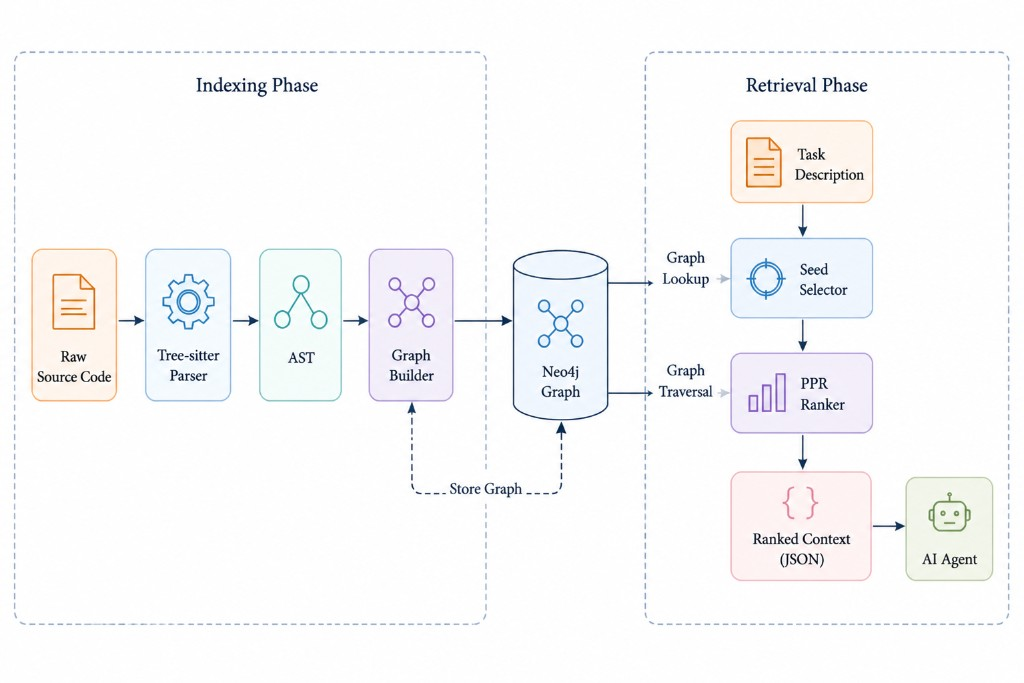
\includegraphics[width=\linewidth]{assets/pipeline_architecture.png}
    \caption{Overview of the CodeGraph indexing and retrieval pipeline. The indexing phase builds the repository graph offline; the retrieval phase ranks context per query for the AI agent.}
    \label{fig:pipeline-architecture}
\end{figure}

The central design assumption is that lexical and structural evidence play complementary roles in retrieval. The task description provides the initial relevance signal through identifiers and keyword matches, while Personalized PageRank propagates that signal over the dependency graph to identify structurally supported regions of the codebase. Regions reinforced by multiple structural connections gain prominence, whereas weakly connected or isolated matches lose influence in the final ranking.

This decomposition also supports practical retrieval performance. Parsing and graph construction are carried out before query execution, while per-query retrieval operates over an already constructed graph and is dominated primarily by the ranking computation.

\subsection{Source Code Parsing}

Graph-based retrieval requires an explicit structural representation of the repository. A source file, in its raw textual form, does not yet expose the code units and relationships needed for graph construction. CodeGraph parses Python source files into a typed entity model using Tree-sitter. 

A central design question is the level of granularity at which entities should be extracted. CodeGraph adopts a four-entity model consisting of files, classes, functions, and methods. This choice provides a practical middle ground: it captures the units through which Python code is typically organized and referenced, while preserving a graph size that remains suitable for efficient retrieval. Each entity receives a qualified name, which acts as a repository-wide identifier (e.g., \texttt{path/to/file.py::ClassName}).

Import statements express cross-file dependencies. Import resolution addresses this by mapping each resolvable import to a file on disk and converting it into an edge between the importing file and the imported module. Call resolution converts function call expressions into edges by determining which definition each call site refers to, resolving calls via a three-level strategy in descending order of confidence (imported definitions, intra-file definitions, and unique repository-wide definitions). Ambiguous calls are omitted to favor precision over misleading graph pathways.

\subsection{Graph Construction}

CodeGraph stores the extracted entities as a weighted property graph in Neo4j. Nodes correspond to parsed code entities and edges encode structural relationships between them. This graph is the central data structure of the system.

The graph schema mirrors the four-entity representation. Structural relationships between these entities are represented through four edge types: \texttt{CONTAINS}, \texttt{CALLS}, \texttt{IMPORTS}, and \texttt{INHERITS\_FROM}. Together, these node and edge types capture the main structural patterns of a Python codebase. \Cref{fig:graph-schema} illustrates how these relationships fit together.

\begin{figure}[htbp]
    \centering
    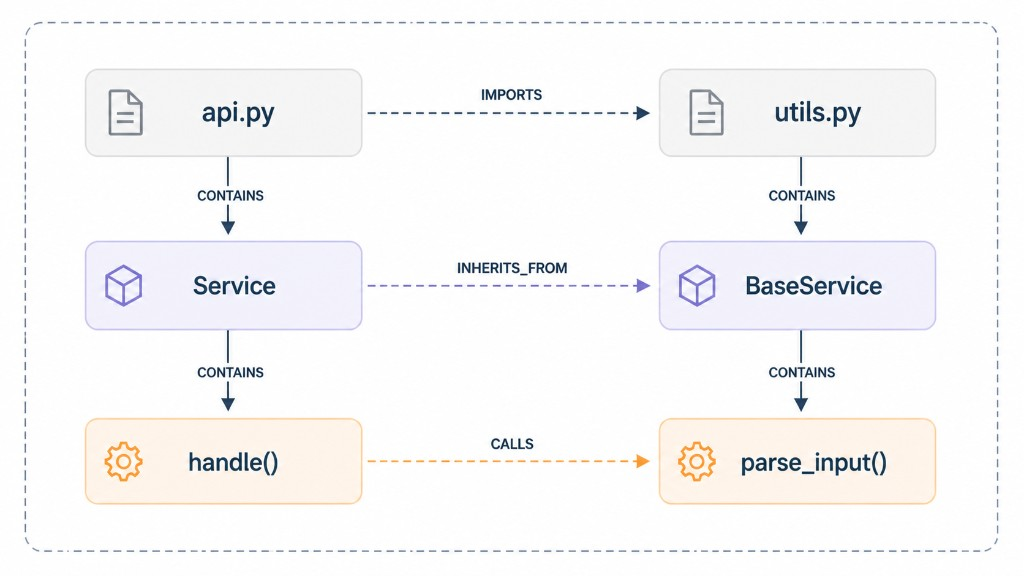
\includegraphics[width=\linewidth]{assets/graph_schema.png}
    \caption{CodeGraph property-graph schema. Nodes represent files, classes, methods, and functions; \texttt{CONTAINS} nests entities within a module, \texttt{IMPORTS} links modules, \texttt{INHERITS\_FROM} records class extension, and \texttt{CALLS} connects invocations.}
    \label{fig:graph-schema}
\end{figure}

All edges are initially created with a uniform base weight of 1.0. During the ranking phase, these weights are updated dynamically based on an Inverse Document Frequency (IDF) mechanism, which attenuates connections to ubiquitous utility hubs while preserving weights for highly specific dependencies.
